%\VignetteIndexEntry{CGHcall}
%\VignetteDepends{}
%\VignetteKeywords{Calling aberrations for array CGH tumor profiles.}
%\VignettePackage{CGHcall}

\documentclass[11pt]{article}

\usepackage{amsmath}
\usepackage[authoryear,round]{natbib}
\usepackage{hyperref}


\usepackage{c:/Data/Programs/R/R-2.7.0dev/share/texmf/Sweave}
\begin{document}

\setkeys{Gin}{width=0.99\textwidth}

\title{\bf CGHcall: Calling aberrations for array CGH tumor profiles.}

\author{Sjoerd Vosse and Mark van de Wiel}

\maketitle

\begin{center}
Department of Pathology\\
VU University Medical Center
\end{center}

\begin{center}

{\tt mark.vdwiel@vumc.nl}
\end{center}


\tableofcontents

%%%%%%%%%%%%%%%%%%%%%%%%%%%%%%%%%%%%%%%%%%%%%%%%%%%%%%%%%%%%%%%%%%%%%%%%%%%
\section{Overview}

CGHcall allows users to make an objective and effective classification of their aCGH data into copy number states (loss, normal, gain or amplification). This document provides an overview on the usage of the CGHcall package. For more detailed information on the algorithm and assumptions we refer to the article \citep{CGHcall} and its supplementary material. As example data we attached the first five samples of the Wilting dataset \citep{Wilting}. After filtering and selecting only the autosomes 4709 datapoints remained.

\section{Example}

In this section we will use CGHcall to call and visualize the aberrations in the dataset described above. First, we load the package and the data:

\begin{Schunk}
\begin{Sinput}
> library(CGHcall)
> data(WiltingData)
> Wilting <- cghRaw(WiltingData)
\end{Sinput}
\end{Schunk}

\noindent
Next, we apply the {\tt preprocess} function which:
\begin{itemize}
\item removes data with unknown or invalid position information.
\item shrinks the data to {\tt nchrom} chromosomes.
\item removes data with more than {\tt maxmiss} \% missing values.
\item imputes missing values using {\tt impute.knn} from the package {\tt impute} \citep{Impute}.
\end{itemize}

\begin{Schunk}
\begin{Sinput}
> cghdata <- preprocess(Wilting, maxmiss = 30, nchrom = 22)
\end{Sinput}
\begin{Soutput}
Changing impute.knn parameter k from 10 to 4 due to small sample size.
Cluster size 3552 broken into 984 2568 
Done cluster 984 
Cluster size 2568 broken into 1509 1059 
Cluster size 1509 broken into 653 856 
Done cluster 653 
Done cluster 856 
Done cluster 1509 
Done cluster 1059 
Done cluster 2568 
\end{Soutput}
\end{Schunk}

To be able to compare profiles they need to be normalized. In this package we provide very basic global median or mode normalization. Of course, other methods can be used outside this package. This function also contains smoothing of outliers as implemented in the DNAcopy package \citep{DNAcopy}. Furthermore, when the proportion of tumor cells is not 100\% the ratios can be corrected. See the article and the supplementary material for more information on cellularity correction \citep{CGHcall}.

\begin{Schunk}
\begin{Sinput}
> tumor.prop <- c(0.75, 0.9, 0.8, 1, 1)
> norm.cghdata <- normalize(cghdata, method = "median", cellularity = tumor.prop, 
+     smoothOutliers = TRUE)
\end{Sinput}
\begin{Soutput}
Applying median normalization ... 
Smoothing outliers ... 
Adjusting for cellularity ... 
Cellularity sample 1 :  0.75 
Cellularity sample 2 :  0.9 
Cellularity sample 3 :  0.8 
Cellularity sample 4 :  1 
Cellularity sample 5 :  1 
\end{Soutput}
\end{Schunk}

The next step is segmentation of the data. This package only provides a simple wrapper function that applies the {\tt DNAcopy} algorithm \citep{DNAcopy}. Again, other segmentation algorithms may be used. To save time we will limit our analysis to the first two samples from here on.

\begin{Schunk}
\begin{Sinput}
> norm.cghdata <- norm.cghdata[, 1:2]
> seg.cghdata <- segmentData(norm.cghdata, method = "DNAcopy")
\end{Sinput}
\begin{Soutput}
Start data segmentation .. 
Analyzing: Sample.1 
Analyzing: Sample.2 
\end{Soutput}
\end{Schunk}

Now that the data have been normalized and segments have been defined, we need to determine which segments should be classified as losses, normal, gains or amplifications.

\begin{Schunk}
\begin{Sinput}
> result <- CGHcall(seg.cghdata)
\end{Sinput}
\begin{Soutput}
EM algorithm started ... 
Calling iteration 1 :
 [1]  2.000000e+00 -3.775517e+03 -8.557179e-01 -2.760899e-01  1.440993e-02
 [6]  3.037901e-01  1.107552e+00  3.044664e-05  9.765269e-02  5.106221e-02
[11]  1.552210e-01  1.009465e-04
Calling iteration 2 :
 [1]  2.000000e+00 -3.774833e+03 -8.664196e-01 -2.694464e-01  1.896237e-02
 [6]  3.000849e-01  1.100138e+00 -4.573000e-06  9.874358e-02  4.889779e-02
[11]  1.613372e-01  1.010569e-04
EM algorithm done ...
FINISHED!
Total time: 1 minutes
\end{Soutput}
\end{Schunk}

\pagebreak
\noindent
To visualize the results per profile we use the {\tt plotProfile} function:

\begin{center}
\begin{Schunk}
\begin{Sinput}
> plot(result[, 1])
\end{Sinput}
\begin{Soutput}
Plotting sample AdCA10 
\end{Soutput}
\end{Schunk}
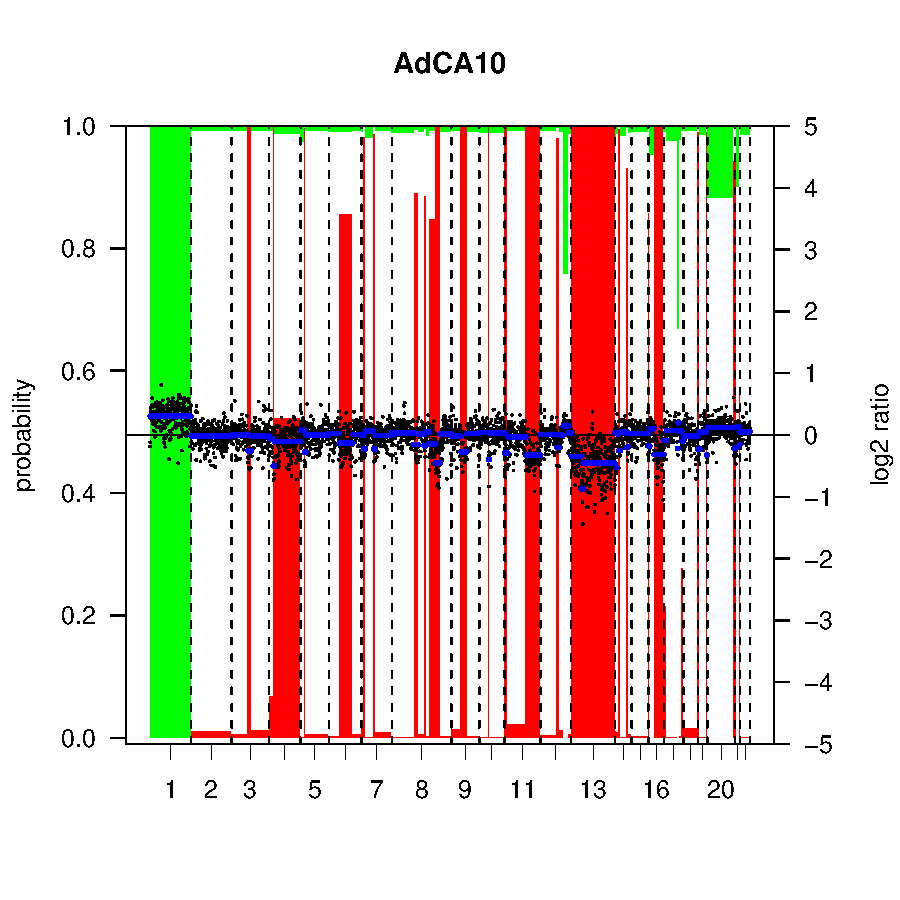
\includegraphics{CGHcall-006}
\end{center}

\pagebreak
\begin{center}
\begin{Schunk}
\begin{Sinput}
> plot(result[, 2])
\end{Sinput}
\begin{Soutput}
Plotting sample SCC27 
\end{Soutput}
\end{Schunk}
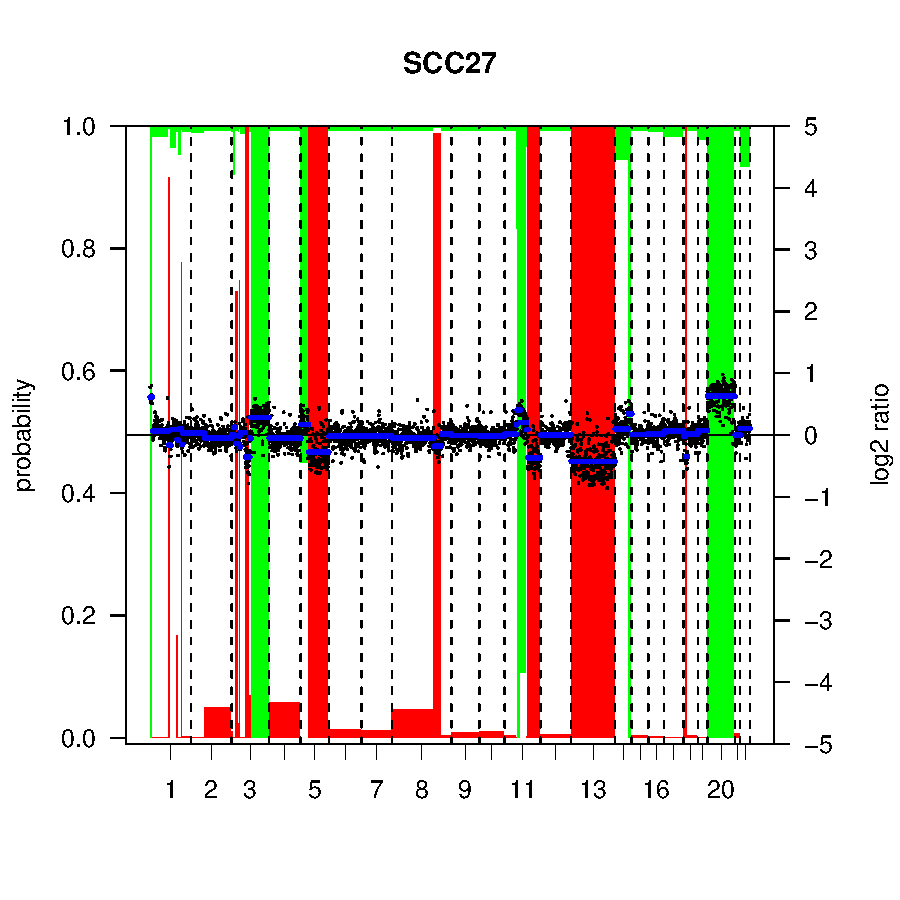
\includegraphics{CGHcall-007}
\end{center}

\pagebreak
\noindent
Alternatively, we can create a summary plot of all the samples:

\begin{center}
\begin{Schunk}
\begin{Sinput}
> summaryPlot(result)
\end{Sinput}
\begin{Soutput}
Adding sample AdCA10 to summary plot.
Adding sample SCC27 to summary plot.
\end{Soutput}
\end{Schunk}
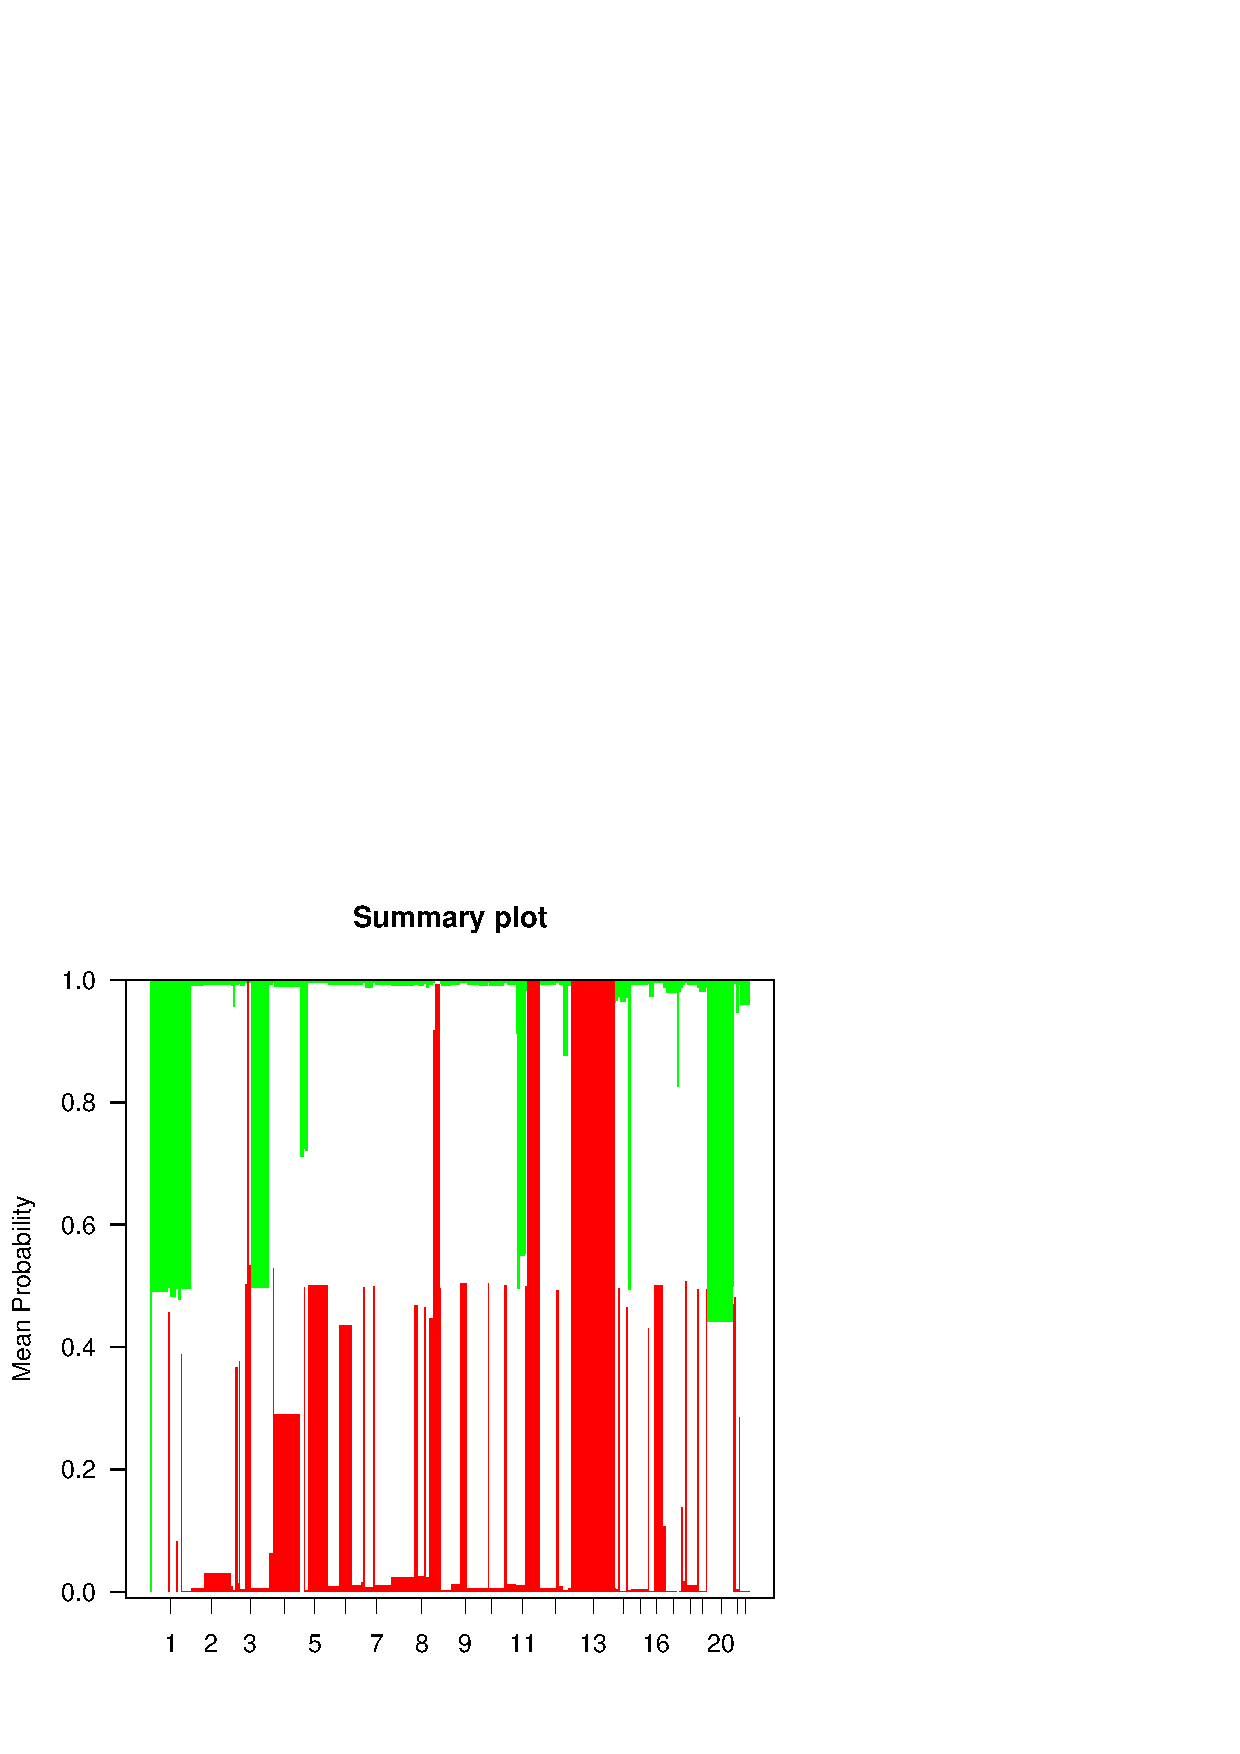
\includegraphics{CGHcall-008}
\end{center}

\pagebreak
%\newpage
\bibliographystyle{apalike}
\bibliography{CGHcall}

\end{document}
